%auto-ignore
\documentclass[preview=false]{standalone}

\usepackage{graphics,graphicx,xcolor}
\usepackage{standalone}
\usepackage{tikz}
\usetikzlibrary{automata, arrows.meta, positioning}

\definecolor{rouge}{RGB}{255,77,77}
\definecolor{vert}{RGB}{0,178,102}
\definecolor{jaune}{RGB}{255,255,0}
\definecolor{violet}{RGB}{208,32,144}
\definecolor{orange}{RGB}{255,140,0}
\definecolor{bleu}{RGB}{0,0,205}

 
\begin{document}
 
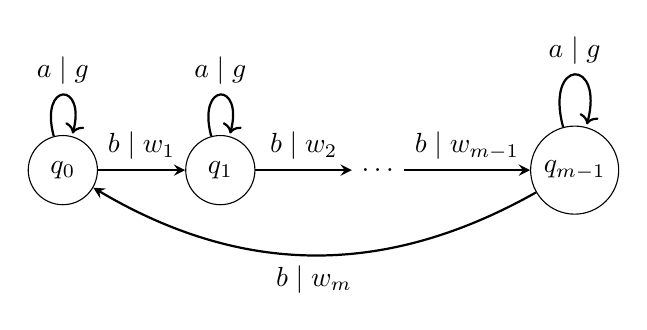
\begin{tikzpicture}[node distance = 3cm, on grid, auto]
    \node (q0) [state] at (0,0) {$q_0$};
    \node (q1) [state] at (2,0) {$q_1$};
    \node (q2) at (4,0) {$\dots$};
    \node (qn) [state] at (6.5,0) {$q_{m-1}$};


\path [-stealth, thick]
    (q0) edge node {$b\mid w_1$}   (q1)
    (q1) edge node {$b\mid w_2$}   (q2)
    (q2) edge node {$b \mid w_{m-1}$}   (qn)
    (qn) edge [bend left] node {$b \mid w_m$}   (q0)
    (q0) edge [loop above]  node {$a\mid g$}()
    (q1) edge [loop above]  node {$a \mid g$}()
    (qn) edge [loop above]  node {$a \mid g$}();

\end{tikzpicture}


\end{document}
